\qns{Shrinking Transistor Size [OPTIONAL]}

\qcontributor{Regina Eckert}
Moore's Law is a 1965 observation by Fairchild Semiconductor Research and Development Lab's director, Gordon Moore, that the number of transistors on an integrated circuit chip doubles every 1.5-2 years. This observation has dominated the computer industry into modern day, where we now have sophisticated processes to create transistors that have a smallest feature size that is 10 \si{\nano\meter} across.

\begin{enumerate}
	\qitem Given that silicon atoms in a lattice are separated by $\approx 0.543 \si{\nano\meter}$, how many silicon atoms thick is a $10 \si{\nano\meter}$ feature?
	
	\sol{We have a total length of 10 nm that is composed of atoms that are separated by 0.543 nm. The number of atoms $n = \frac{total~length}{distance~per~atom} = \frac{10~nm}{0.543~nm} = 18.4162$. A 10 nm feature is approximately 18 atoms thick.
	}

	\qitem Here is a transmission electron microscope (TEM) image of a FINFET transistor from Intel, where you can see the silicon atoms in an ordered lattice.
	
	\begin{figure}[H]{
			\centering
			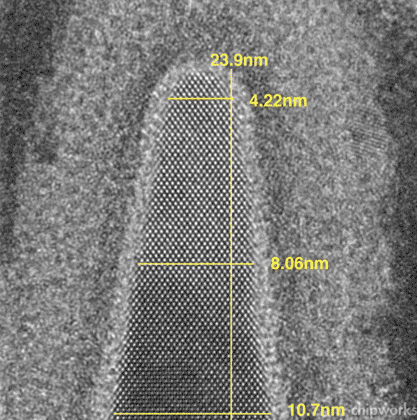
\includegraphics[width=0.3\textwidth]{q_moores_law/tem_silicon_image.png}
			\caption{TEM Image of Intel FINFET Transistor}
			\vspace{-5mm}}
		\label{fig:TEM}
	\end{figure}
\end{enumerate}

	How many atoms across is the feature where it is $4.22 \si{\nano\meter}$ wide?
	\sol{There are 12 atoms (white dots) across the feature.}
	
	\qitem If the most recent 10 \si{\nano\meter} technology was released in 2017, by applying Moore's Law, when would we expect features that are 1 silicon atom wide? Assume that the feature size is reduced by half every time the number of transistors doubles.
	
	\sol{We can write out the equation for the number of transistors on a chip in year $y_n$ relative to previous year $y_0$ as 
		\begin{equation}
		N_{y_n} = N_{y_0}*2^{(y_n-y_0)/t_{double}},
		\end{equation}
		
	where $t_{double}$ is the number of years it takes for the number of transistors to double.
	
	If the feature width $W$ is halved every time the number of transistors doubles, then we can write the equation for the width in future year $y_n$ as 
	\begin{equation}
	W_{y_n} = \frac{W_{y_0}}{2^{(y_n-y_0)/t_{double}}}.
	\end{equation}
	
	Plugging in for $W_{y_0} = 10nm$, $y_0 = 2017$, and $W_{y_n} = 0.543 nm$, and rearranging, we get:
	\begin{equation}
	2^{(y_n-y_0)/t_{double}}= \frac{W_{y_0}}{W_{y_n}}
	\end{equation}
		
	\begin{equation}
	2^{(y_n-2017)/t_{double}}= \frac{10nm}{0.543nm} = 18.4162
	\end{equation}
	
	\begin{equation}
	\frac{y_n-2017}{t_{double}}\text{log}(2)= \text{log}(18.4162)
	\end{equation}
	
	\begin{equation}
	\frac{y_n-2017}{t_{double}}= \text{log}(18.4162)/\text{log}(2) = 4.2029
	\end{equation}
	
	\begin{equation}
	y_n= 4.2029*t_{double}+2017
	\end{equation}
	
	If $t_{double}=1.5$, $y_n = 2023$ and if $t_{double}=2$, $y_n = 2025$. It will take between 6-8 years to reach a feature that is only 1 silicon atom wide if we halve the transistor feature width every 1.5-2 years.
	
	}
	 
	\qitem Do you think Moore's Law can continue forever? Why or why not?
	
	\sol{ No, Moore's Law cannot continue forever. Among other reasons, we cannot create a reliable process that consistently creates features that are 1 atom wide. Also, our use of the materials assumes that the features have some thickness, and that assumption breaks down when there are such few atoms across a device.
	}
	
	